\documentclass{article}

\usepackage[a4paper,left=18mm,right=18mm,top=20mm,bottom=18mm]{geometry}
\usepackage[italian]{babel}

\usepackage{titling}
\usepackage{graphicx}
\usepackage{subcaption}
\usepackage{float}
\usepackage{hyperref}


\title{Breve report sui risultati ottenuti tesi}
\author{David Guzman Piedrahita and Marco Vinciguerra}
 
\begin{document}
\maketitle        
\section{Introduzione e reti neurali utilizzate}
Per studiare la potenziale relazione tra ammoniaca e particolato, sono state utilizzate
diverse strategie di machine learning, in modo di trovare una combinazione di approcci
che rifletta, nel modo più accurato possibile, il comportamento e le interazioni tra le due 
sostanze in questione, anche in relazione ad altre variabili di inquinamento e meteorologiche.
\\In particolare, sono state utilizzate diverse tipologie di rete neurali LSTM (long-short term memory),
che sono adatte a modellizzare fenomeni che dipendono da stati precedenti del sistema
in quanto permettono di possedere l'informazione degli
istanti temporali precedenti. Le diverse strategie
che sono state valutate, comprendono metodologie per gestire la mancanza di dati nel dataset, e metodologie
per migliorare il rendimento dei modelli, stabilizzandolo e rimuovendo dati superflui.  
\section{Regressori}
Sono stati utlizzati dati provenienti da diverse centraline meteorologiche e di inquinamento in tutta la Lombardia.
\\Usando, per esempio, i dati di Moggio che vanno dal 2014 al 2020, possiamo ottenere risultati che sottolineano una 
forte relazione del particolato rispetto all'ammoninaca, in concomitanza di altri dati  
Wind\_speed, Wind\_direction (in gradi), quadrante della 
velocità del vento, Temperature e Rainfall. 
Infatti,usando per la creazione del mdoelli dati dal 2014 al 2019 e per la 
validazione tutto il 2020. Otteniamo un notevole inseguimento della previsione  rispetto ai dati reali, 
usando dati di 5 giorni successivi per determinare l'andamento del sesto giorno.
\section{Training}
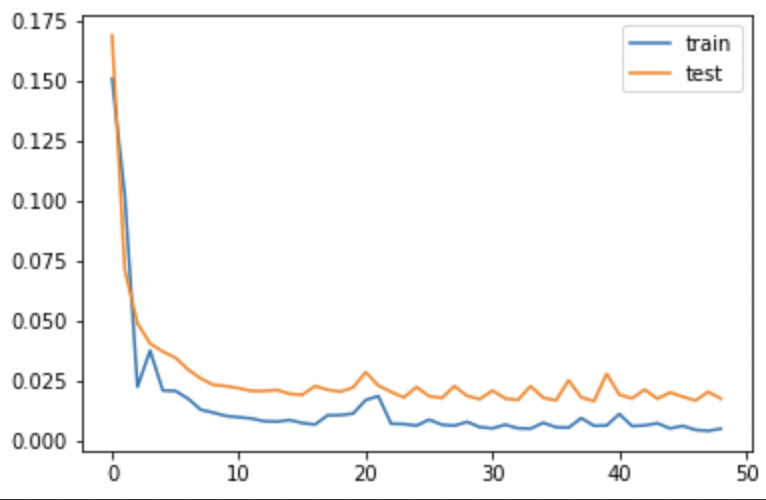
\includegraphics[scale = 0.5]{Immagini/Training.PNG}
\section{Regressione tramite reti neurali}
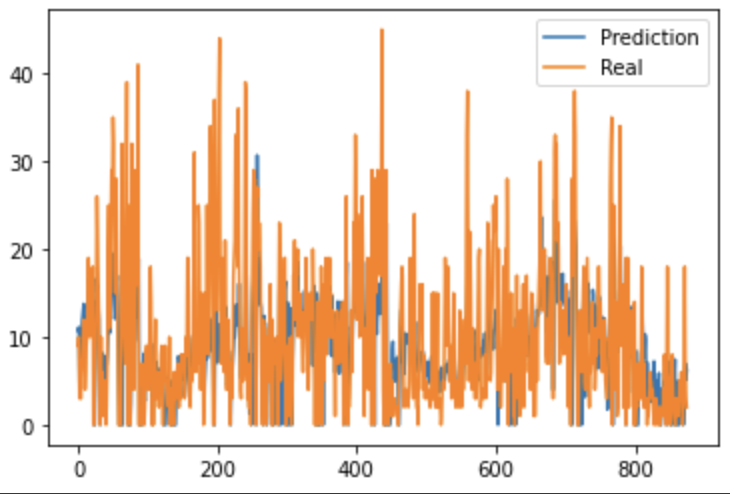
\includegraphics[scale = 0.5]{Immagini/Regressione1.PNG}
\end{document} 
